\subsection{Ngspice Script Specifications and Simulation Goals}
\hspace{12pt} Given that there exist a very extensive amount of different OP-AMPs, in this laboratorial session we were given a specific model - the 741 OP-AMP - whose internal composition is described in the first lines of the Ngspice script. The 741 OP-AMP is comprised of: 

\begin{itemize}
	\item{2 Capacitors}
	\item{5 Diodes}
	\item{1 Voltage Controlled Voltage Source (VCVS)}
	\item{1 Current Controlled Current Source (CCCS)}
	\item{2 Voltage Controlled Current Sources (VCCS)}
	\item{1 Current Controlled Voltage Source (CCVS)}
	\item{2 NPN Transistors}
	\item{9 Resistors}
	\item{6 Independent Voltage Sources}
	\item{1 Independent Current Source}
\end{itemize} 

By using this OP-AMP and using the circuit architecture described in Figure \ref{fig:circuit}, we used the Ngspice script provided, we were able to analyze and tweak the values of the resistors and capacitors in order to achieve our set goals, these included:

\begin{enumerate}
	\item{Bringing the central frequency of the bandpass filter as close as possible to 1kHz}
	\item{Getting a gain value close to 40dB (which is equivalent to a gain of 100)}
	\item{Achieving points 1 and 2 whilst also adhering to the strict component list available (3 $1k\Omega$, $10k\Omega$, and $100k\Omega$ resistors and 3 $220nF$ and $1\mu F$ capacitors)}
	\item{Maximizing the merit value of the circuit}
\end{enumerate}

After \textit{several} attempts, we arrived at the following values for the components: 

\begin{itemize}
	\item{$R_1 = 10k\Omega$}
	\item{$R_2 = 1k\Omega$}
	\item{$R_3 = 150k\Omega$ (1 $100k\Omega$ resistor in series with a branch of 2 parallel $100k\Omega$ resistors)}
	\item{$R_4 = 500\Omega$ (2 $1k\Omega$ resistors in parallel)}
	\item{$C_1 = 265.0602409638554nF$ (3 branches in series composed of: 2 $1\mu F$ parallel capacitors, 2 $220nF$ parallel capacitors and 1 $1\mu F$ capacitor)}
	\item{$C_2 = 220nF$}
\end{itemize} 
\pagebreak
\subsection{Frequency Response}

\hspace{12pt} Using these values, we can perform a frequency response analysis and obtain the following plots for the magnitude and phase of the output voltage:

\begin{figure}[h!]
	\centering
	\subfigure[]{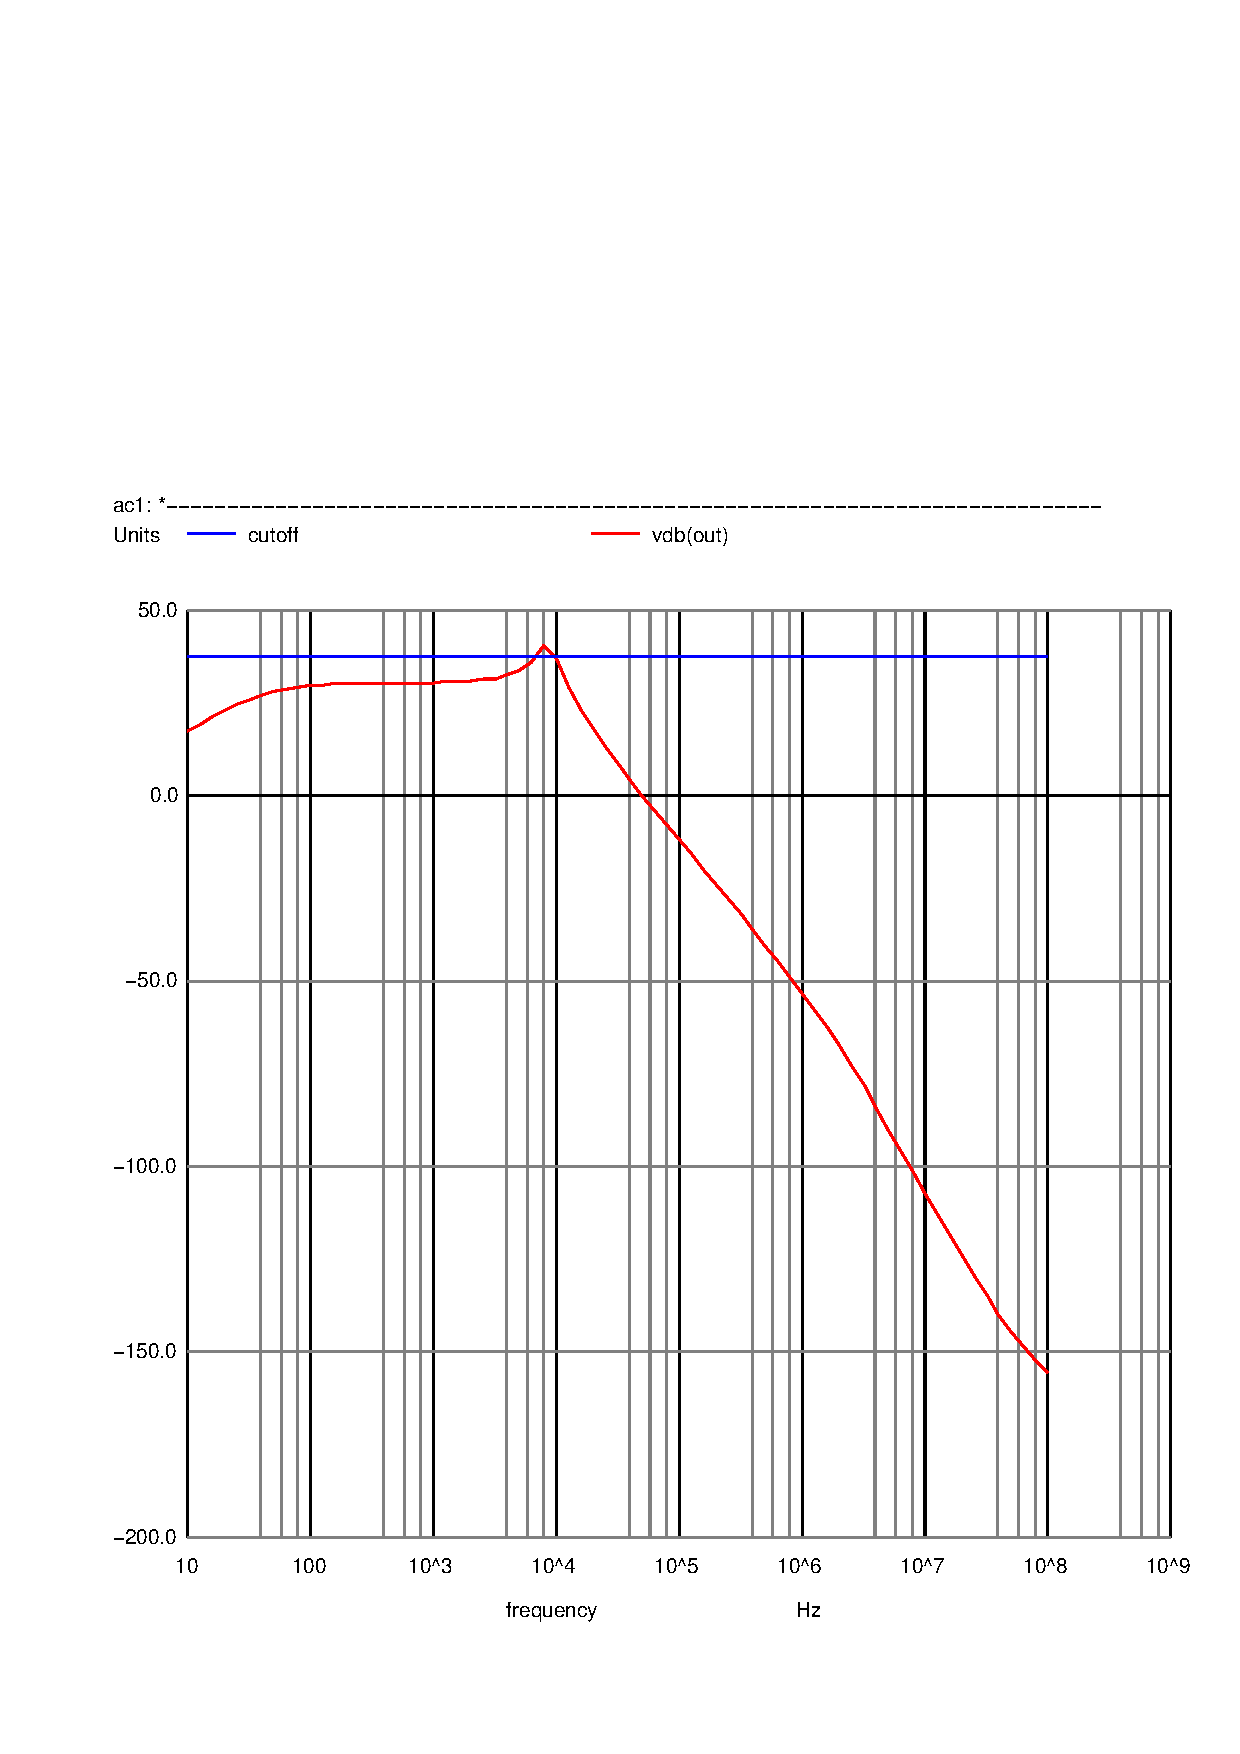
\includegraphics[width=0.49\textwidth, trim={0 2cm 0 8cm}, clip]{vout_mag.pdf}}
	\subfigure[]{\includegraphics[width=0.49\textwidth, trim={0 2cm 0 8cm}, clip]{vout_ph.pdf}}
	\caption{(a) Magnitude plot (b) Phase plot of the frequency response output}
	\label{fig:gain_sim}
\end{figure}

Analyzing the plot in Figure \ref{fig:gain_sim}a, we can define the cutoff frequencies $f_1$ and $f_2$ using the same method as in the previous section, computing these values, along with the gain, input and output impedances at a frequency of 1kHz, we obtain: 

\begin{figure}[h]
	\centering
	\begin{tabular}{|c|c|}
		\hline
		\input{out_tab.tex}
	\end{tabular}
	\caption{Simulation results}
	\label{fig:results_sim}
\end{figure}

As we can see, both the gain and the central frequency are close to the intended values (the gain is represented in linear units and given that $40dB = 20log_{10}(G) \iff G = 10^{40/20} = 100$, a gain close to 100 is optimal), the main reason for the low merit value is the huge cost of the OP-AMP component (13323.2920387 MU) which, when compared to the cost of the other components used (316.66MU), drops the merit value by 4 orders of magnitude. 
\pagebreak
\subsection{Output Signal}
\hspace{12pt} Lastly, it is interesting to look at the output signal given by the bandpass amplifier circuit (Figure \ref{fig:output_sim}). As is possible to see, there is little to no distortion in the signal as the shape closely resembles the sinusoidal wave of the input voltage, this is an advantage for many applications, including audio speakers.

\begin{figure}[h]
	\centering
	\includegraphics[width=0.4\textwidth, trim={0 2cm 0 8cm}, clip]{vout.pdf}
	\caption{Output signal plot}
	\label{fig:output_sim}
\end{figure}

